\section{Systemets funktionelle krav}
Systemets input er patienternes kropshældning, dvs. hvor meget vedkommende svajer i normal kropsstilling (anatomisk udgangsposition) og under udførelse af en bestemt øvelse. Systemet skal kunne konvertere informationer vedrørende patienternes kropshældning til visuel og sensorisk feedback, samt give et digitalt output i form af grafer. Selve systemet skal anvendes til selvtræning i hjemmet, hvor to sværhedsgrader kan anvendes. Dette gøres ved anvendelse af systemet  under den normale kropsstilling og udvalgte træningsøvelse. Denne træningsøvelse er valgt for i højere grad at udfordre patienternes balance, da kropsvægten fordeles anderledes ved øvelsen ift. den normale kropsstilling. Hvis patienternes kropshældning overskrider den normale grænse for krops svaj, der er seks til syv grader i lateral retning, vil den visuelle og sensoriske feedback gøre patienten opmærksom på dette, samt retning af hældningen. Således kan systemet registrere, hvis patienten er i risiko for at falde og dermed fungere som en hjælp for apopleksipatienter ved at gøre dem opmærksomme på deres kropshældning. Udover den visuelle og sensoriske feedback har systemet et digitalt output, så patienternes øvelsesresultater kan behandles og gemmes på en computer. Den digitale del af systemet henvender sig derfor til fagkyndigt personale, der på denne måde kan følge med i udviklingen af patienternes balance. 


De funktionelle krav:
\begin{itemize}
\item Systemet skal være brugervenligt, så det kan anvendes af apopleksipatienter og fagkyndigt personale.
\item Systemet skal kunne måle patienternes kropshældning og konvertere det til visuel og sensorisk feedback, samt et digitalt output.
\item Systemet skal kunne give visuel og sensorisk feedback til patienten ved forskellig hældningsgrad ift. hvilken sværhedsgrad patienten vælger.
\item Systemet skal kunne give et digitalt output, så det er muligt at behandles og gemme patienternes data på en computer.
\item Systemet skal indeholde en "switch" knap, så patienterne kan skifte mellem de to sværhedsgrader.
\end{itemize}

\section{Systemets opbygning}
\begin{figure}[H]
\centering
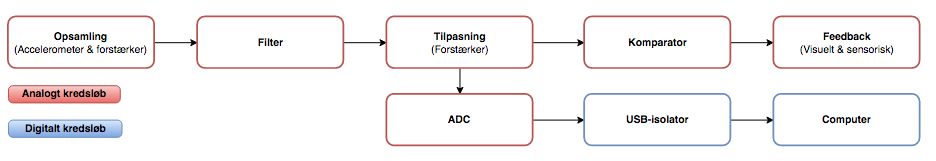
\includegraphics[scale=0.5]{figures/Blokdiagram.jpg}
\caption{Her ses et blokdiagram af systemets opbygning}
\label{Blokdiagram}
\end{figure}

Det biologiske signal der opnås fra accelrometeret skal forstærkes, eftersom signalerne der opfanges er små og det vil derfor gøre filtreringen mere præcis ved at forstærke signalet. Herefter benyttes et højpas filter for at frasortere den støj der kommer fra tyngdekraften. \fxnote{Der skal tilføjes noget om højpas filter ligesom det der står ved lavpas filter} Lavpasfiltret anvendes for at frasortere støj fra frekvenser over 45 Hz. Grunden til disse frekvenser kan frasorteres er, at det signal som måles på ligger under 45 Hz. Efter filtreringen af signalet benyttes en variabel forstærker, for at tilpasse signalets amplitude til ADC’en og komparatoren. Signalet ledes herefter videre i et analogt og digitalt kredsløb. I det analoge kredsløb kommer signalet først gennem en komparator, som skal sammenligne signalet der optages, så den rigtige feedback kan gives til patienten ift. valgt sværhedsgrad. Feedbacken gives til patienten i form af dioder og vibratorer. I det digitale kredsløb, ledes signalet ind i en ADC, som konverterer det analoge signal til et digitalt signal. Herefter ledes det digitale signal ind i en USB-isolator, så der ikke opstår lækstrømme og for at sikre patientens sikkerhed. Til sidst overføres det digitale signal til en computer, hvor signalet herefter kan databehandles og gemmes.


%Systemet har til formål at hjælpe apopleksipatienter med rehabiliteringen af deres balancefunktion i hjemmet. Dette gøres ved en træningøvelse, hvor systemet skal gå ind og advare patienten om risiko for fald under øvelsen. Måden patienten skal advares, er ved at måle kropshældningen under forsøget. Hvis patienten kommer til at hælde for meget, skal der være et biofeedback system, som advarer patienten om hvilken retning de er ved at falde til højre eller venstre. Feedbacksystemet udgøres af en visuel og en sensorisk del. %Der benyttes to feedback dele, da brugeren af systemet kan være dårligt seende, eller have kognitive problemer, som kan gøre det svært at opfange kun en form for feedback.   
%Derudover skal der være en digital feedback, som kan gemmes, så øvelsens resultater kan ses igen. 